 \documentclass[11pt]{article}
 \usepackage[italian]{babel}

% \usepackage{fontspec}
% \setmainfont{Calibri}

 %setting margins
 \usepackage[margin=2cm,nohead]{geometry}
 \usepackage{circuitikz}
 \usepackage{graphicx}
 \usepackage{tikz}
 \usepackage{booktabs}
 \usepackage{amsmath}
 \usepackage{amsfonts}
 \usepackage{hyperref}
\usepackage{titling}
 \usepackage{textcomp}

 \ctikzset{bipoles/thickness=1.2}
 \setlength{\droptitle}{-11ex}
 \title{Analisi di un circuito RLC serie in regime sinusoidale}
 \author{Autori: Niccolò Zanotti mat. 970919, Michael Mancini mat. 987056}
 \date{Data di svolgimento: 01/06/2022}

 \begin{document}

  \maketitle

  \section{Abstract}
    In questa esperienza di laboratorio si è analizzato il comportamento di un circuito RLC serie sottoposto a una tensione
in regime sinusoidale con pulsazione variabile.
In particolar modo si è cercato di stimare il valore della frequenza di risonanza, andando a confrontare il comportamento
del circuito per valori della frequenza prossimi
al valore cercato per poi, acquisendo e analizzando i dati relativi alla tensione in entrata e nei rami, verificare
l’andamento atteso dell’ampiezza della tensione.

Uno dei valori della frequenza di risonanza ottenuto per via sperimentale mediante l'utilizzo dei parametri del fit dell'ampiezza
della tensione sulla resistenza risulta essere $f = (18.95 \pm 0.05) kHz$, compatible con il valore
della frequenza di risonanza atteso pari a $f = (19.13 \pm 0.14) kHz$. %% #TODO valuta se scrivere del valore della fase



 \section{Introduzione}
   In un circuito $RLC$ in regime sinusoidale si assiste al fenomeno fisico della risonanza; in particolare, dati i valori
caratteristici di resistenza,induttanza e capacità del circuito, si osserva tale fenomeno in corrispondenza di un preciso
valore di frequenza, detta,appunto, di risonanza. La larghezza della curva di risonanza è legato al valore del cosiddetto
fattore di qualità $Q$ del circuito determinato dai componenti circuitali utilizzate.
È stato utilizzato un generatore di tensione sinusoidale il cui scopo principale è stato quello di indurre oscillazioni
della corrente all'interno circuito e per valutare la sua risposta in frequenza.

La frequenza di risonanza si ha quando la tensione generata ai capi del circuito oscilla con pulsazione
\begin{equation}
    \omega_0 = \frac{1}{\sqrt{L C}}
\end{equation}
In corrispondenza di questo valore il comportamento previsto è che la differenza di potenziale ai capi della
resistenza sia in fase con quella ai capi del generatore e che, inoltre, sia massimizzata l'ampiezza di tali segnali
di tensione.
Tale circuito si classifica tra i filtri di tipo "passa banda", ovvero tra quei dispositivi passivi che permettono il
passaggio di frequenze all'interno di un dato intervallo, la cosiddetta banda passante, ed attenua le frequenze al
di fuori di esso.
% #TODO valuta se mettere osservazione sulla corrente
%poichè in un intorno della frequenza di risonanza, la
%corrente che scorre è maggiore, per poi diminuire di ampiezza a mano mano che ci si allontana dalla condizione sopra citata.
%

 \section{Apparato sperimentale}
   I valori dei componenti, utilizzati per l’esperienza di laboratorio qui illustrata, sono stati collegati in serie sulla breadbord della scheda di acquisizione dati NI Elvis II e sono stati scelti in maniera tale da ottenere un fattore di qualità Q ragionevole.
In particolare si è deciso di utilizzare una resistenza R....., una capacità C......  e un’induttanza L....., caratterizzata da una resistenza interna corrispondente a.... Questi valori sono stati misurati mediante l’utilizzo del multimetro digitale di ELVIS.
Si è tenuta in considerazione, inoltre, la resistenza interna del generatore di valore....., che perciò risulta essere non del tutto trascurabile rispetto alla resistenza totale del circuito analizzato.
I capi di ogni componente, cosi come gli estremi del circuito, illustrato nella Figura 1., sono stati collegati a un canale della scheda per la lettura dei valori di ampiezza e fase della tensione tramite il programma LabView.
Per realizzare questa esperienza di laboratorio sono stati raccolti.....
L’ampiezza, la frequenza e la fase del segnale di tensione utilizzati per l’analisi dati sono stati ottenuti da ogni acquisizione mediante l’utilizzo del subVI “Extract Single Tone Information” del programma Labview, utilizzato per l’acquisizione dei dati.

 \section{Analisi dei risultati}
   \subsection{Osservazione qualitativa degli andamenti}

\begin{figure}[h]
    \centering
    \includegraphics[width=1\textwidth]{../figs/tensione-tempo.pdf}
    \caption{\emph{I grafici mostrano gli andamenti della tensione ai capi dei vari componenti quando il generatore
    oscilla ad una frequenza di $f=16kHz$ e di $f=22kHz$; questi sono valori prossimi a quelli che definiscono la banda del filtro.}}
    \label{fig:tensione-tempo}
\end{figure}

%#TODO scrivere che la risposta infrequenza viene fatta grazie al function genrator di elvis

Una volta realizzato il circuito, ne è stato valutato il comportamento qualitativo. A tal proposito si è valutato visivamente
l'andamento temporale delle differenze di potenziale sui vari elementi circuitali mediante l'utilizzo dell'oscilloscopio digitale disponibile in
laboratorio.
In secondo luogo, per una valutazione a posteriori, sono stati raccolti tali dati tramite la DAQ configurata.
Ciò è stato fatto mantenendo la frequenza del generatore costante. In figura \ref{fig:tensione-tempo} sono
mostrati tali andamenti per due valori significativi di $f$ in quanto vicini ai valori di taglio della frequenza, caratteristici
di questo circuito.
%#TODO commento su come ampiezze della tensione hanno senso e anche la fase dopo la risonanza
l’andamento della tensione sulla resistenza è risultato essere in fase con quello indotto sul generatore, come ci si
aspettava dal punto di vista teorico.


\subsection{Analisi delle ampiezze}

Gli andamenti della tensione ai capi di ciascun componente e del circuito stesso, ottenuti da calcoli svolti dal programma di acquisizione dati Labview al variare della frequenza, sono mostrati nella figura 3.
L’incertezza associata alle tensione è stata ottenuta come la deviazione standard delle misure associate all’ampiezza della tensione agli estremi, che sono perciò posti costanti, ottenendo quindi come valore …..
Qui di seguito sono mostrate le funzioni che descrivono l’andamento del modulo dell’ampiezza ai capi di ciascun componente e il procedimento adottato per ricarvarle viene analizzato con più attenzione nella sezione “Appendice”.

\[
    V_R = \frac{R_rV_0}{\sqrt{{(R_r+R)}^2+{ \left(\omega L - \frac{1}{\omega C}\right)}^2}}
\]
\[
    V_L = \frac{\omega L V_0}{\sqrt{R^2+{ \left(\omega L - \frac{1}{\omega C}\right)}^2}}
\]
\[
    V_C = \frac{\frac{V_0}{\omega C}}{\sqrt{R^2+{ \left(\omega L - \frac{1}{\omega C}\right)}^2}}
\]

\begin{figure}[h]
    \centering
    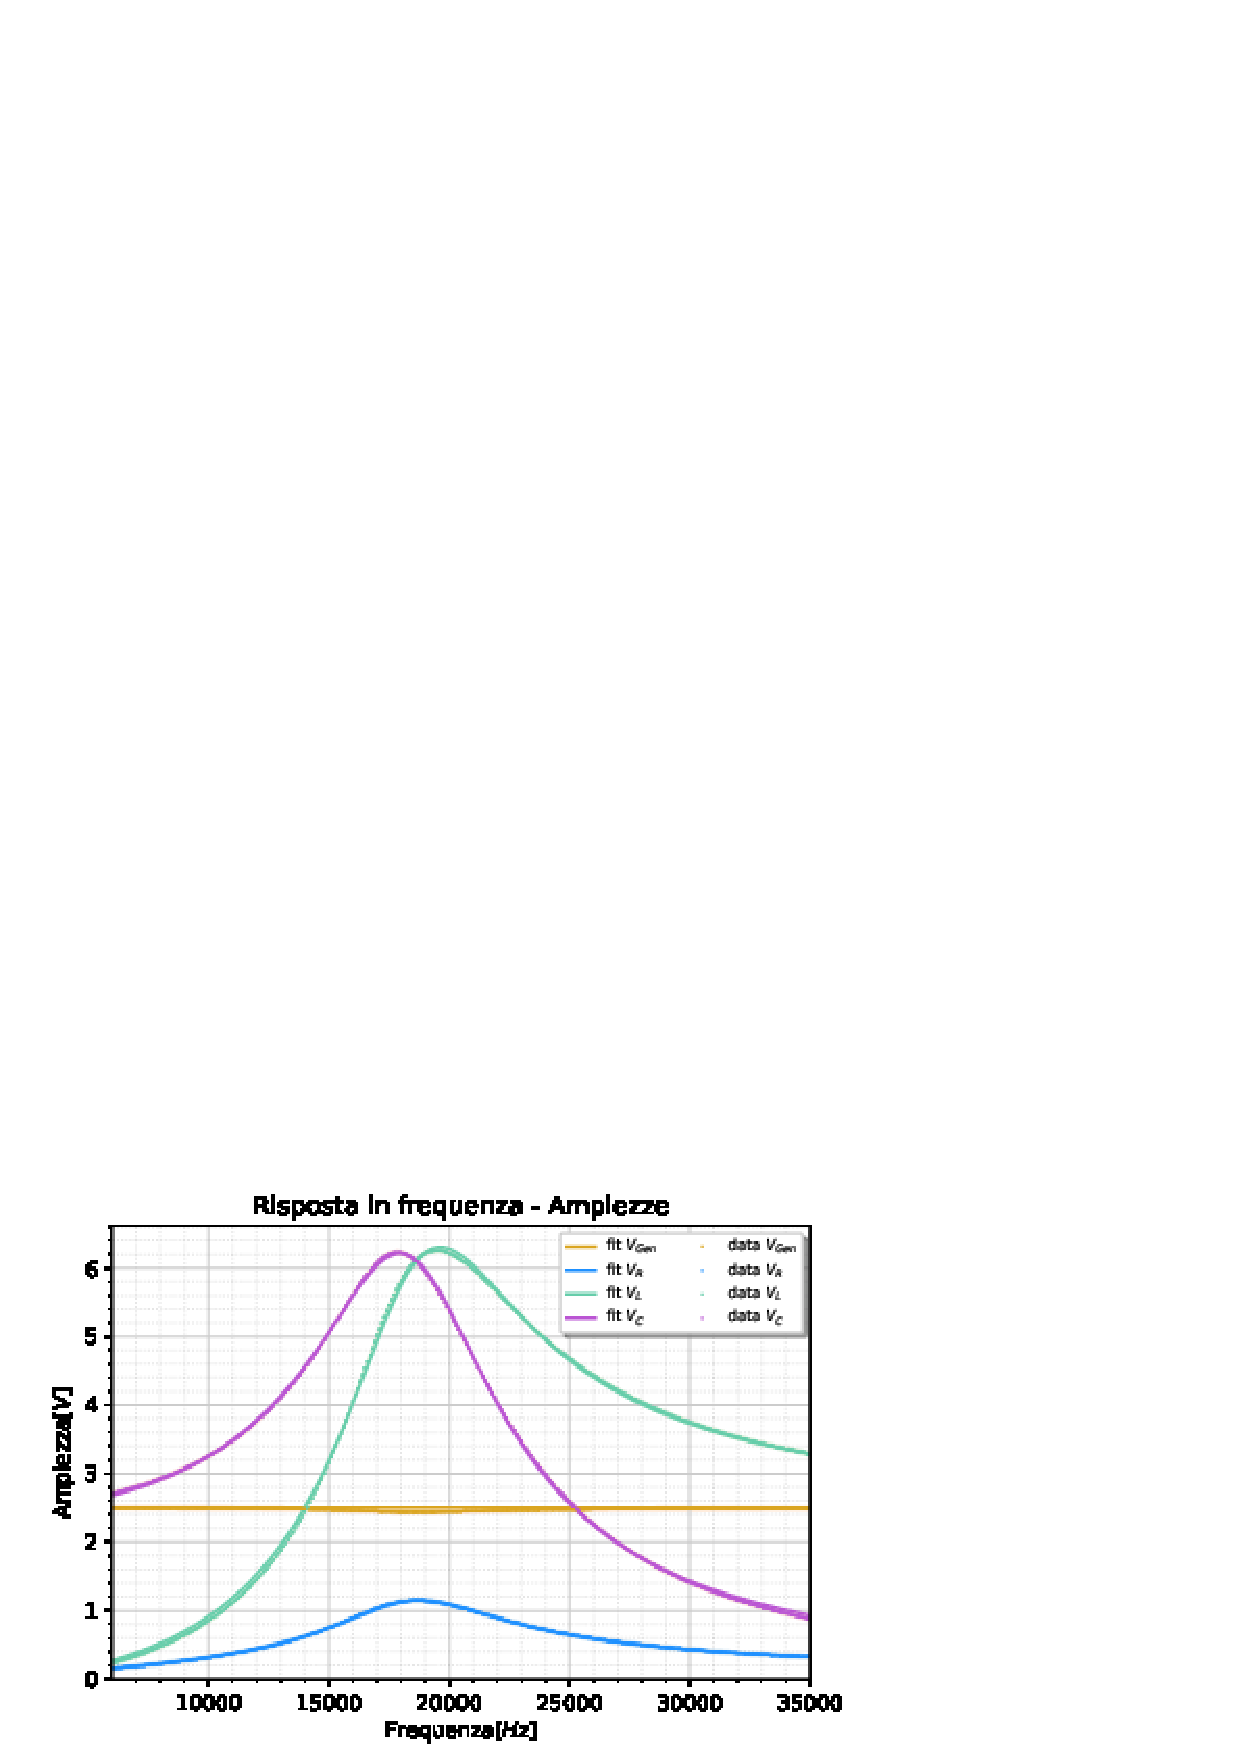
\includegraphics[width=1\textwidth]{../figs/Risposta-in-frequenza-ampiezze.pdf}
    \caption{ampiezze}\label{fig:ampiezzeRLC}
\end{figure}


\begin{figure}[h]
    \centering
    \includegraphics[width=.9\textwidth]{../figs/Risposta-in-frequenza-ampiezza-resistenza.pdf}
    \caption{cambia grafico con nuovi valori fit parametri}\label{fig:ampiezzeR}
\end{figure}




Rr rappresenta la resistenza escludendo però quelle interne a generatore e induttanza, mentre omega indica la pulsazione della tensione applicata.
Andando ad analizzare l’andamento della tensione ai capi di ciascun componente e del circuito stesso, si può notare che l’ampiezza della tensione indotta nel circuito prensenta un picco per valori della frequenza prossimi a quella di risonanza per poi presentare valori più bassi via via che ci si allontana da questa condizione.
Questo effetto è dovuto alla resistenza interna del generatore che provoca una caduta di potenziale proporzionale alla corrente che attraversa il circuito, il cui valore in modulo è massimo proprio in corrispondenza della frequenza di risonanza.
I valori del chi quadro che sono stati ottenuti dai fit sui tre componenti sono...
Si è poi optato di calcolare il valore della frequenza di risonanza con i parametri ottenuti dal fit mediante l’utilizzo dell’equazione 1.
Andando a considerare il fit associato alla resistenza, mostrato in figura 4, i parametri utilizzati sono L=…. e C =….., in questo modo si è controllato se il valore della frequenza di risonanza atteso e calcolato a livello teorico potesse coincidere con quello ottenuto, che è risultato essere di...., dove le incertezze sono state propagate in quadratura.
Un modo alternativo per determinare il valore della frequenza di risonanza è studiare il punto di massimo del grafico relativo all’ampiezza della tensione ai capi della resistenza utilizzata per l’esperienza di laboratorio, ma, non essendo sicuri dell’incertezza sulla misura della tensione, si è deciso di stimare un range di valori.
Preso l’estremo inferiore della barra di errore relativa al punto di massimo estratto dal fit, si sono poi cercati i punti in cui l’estremo superiore della barra di errore corrispondesse a tale valore massimo. In questo modo, però, si è sovrastimata l’incertezza relativa alla frequenza di risonanza, calcolandola come il valore medio di questi due estremi.
Si è ottenuto in questo modo un valore della frequenza di risonanza pari a....
Il valore centrale dell’intervallo scelto è consistente con quanto ottenuto utilizzando i parametri del fit, ma a causa della sovrastima dell’incertezza il risultato può essere considerato poco rilevante.

Parlare eventualmente del valore più alto della resistenza.







\subsection{Analisi delle fasi}

Le funzioni che descrivono gli andamenti attesi delle fasi sono le seguenti:
 \[
     \phi_R = \arctan{\frac{1 - \omega^2 L C}{R \omega C}}
 \]
\[
    \phi_L = \arctan{\frac{1 - \omega^2 L C}{R \omega C}} + \frac{\pi}{2}
\]
 \[
     \phi_C = \arctan{\frac{1 - \omega^2 L C}{R \omega C}} - \frac{\pi}{2}
 \]

\begin{figure}[h]
    \centering
    \includegraphics[width=.9\textwidth]{../figs/Risposta-in-frequenza-fasi.pdf}
    \caption{fasi }\label{fig:fasi}
\end{figure}

Si è poi pensato di estrarre il valore corrispondente a una condizione di fase nulla tra la curva associata alla resistenza e quella del generatore, che risulta essere di..., andando a ripetere lo stesso procedimento analizzando questa volta la curva associata all’induttanza ma, considerando uno sfasamento di 90 gradi, si è ottenuto una misura della frequenza pari a... anch’essa vicina al valore atteso, anche se risulta essere sovrastimata.


 \section{Conclusione}
  

In conclusione il comportamento del filtro è risultato essere in accordo con la teoria.
Per quanto riguarda il fenomeno della risonanza, dall'analisi delle ampiezze per $f_0$ sono stati
ottenuti i valori $f_0 = (18.95 \pm 0.05) kHz$ e $f_0 = (18.80 \pm 0.28)kHz$, mentre
da quella delle fasi $f_0 = (19.10 \pm 0.10)kHz$ e $f_0 = (19.35 \pm 0.15)kHz$ .
Si è ipotizzato che le discrepanze dal valore atteso  $f_0 = (19.13 \pm 0.14) kHz$, dove presenti, siano dovute ai diversi fattori ambientali, primo fra tutti la temperatura
variabile delle componenti della scheda di acquisizione NI ELVIS II, dovuta all’effetto Joule.

È stata inoltre evidenziata un'errata stima iniziale della resistenza totale del circuito, in quanto i valori di tale
grandezza sono risultati sistematicamente superiori in tutti i fit realizzati.
Per avere un'idea di quanto tale valore risulti
superiore a quello atteso di $R_{\text{tot}} = (1172.5 \pm 1.6) \ \Omega$ si riporta tale dato
nel caso del fit più significativo, ossia quello dell'ampiezza di $V_R$, $R =( 2.15 \pm 0.15 )10^3 \ \Omega$.

 \section*{Appendice}
   Come si può notare in Figura 6. le ampiezze nei primi periodi presentano dei picchi più elevati per poi stabilizzarsi a un valore massimo costante, questo comportamento però risulta essere anomalo dal momento che il circuito analizzato in questa esperienza di laboratorio non ha le caratteristiche tipiche di un transiente.
Si è cercato, perciò, di risolvere l’anomalia ripetendo le misure con componenti equivalenti, senza però ottenere nessun risultato positivo nella risoluzione del problema. (L’ho scritto perchè sembra una cosa logica anche se non l’abbiamo fatta).
Dopo vari tentativi, si è ipotizzato che questa anomalia sia dovuta al modo in cui sono raccolti i primi dati dal programma di acquisizione Labview, in particolar modo si è pensato che il problema potesse essere dovuto al trigger del software.

Al fine di studiare il comportamento del circuito analizzato in questa esperienza di laboratorio, si è utilizzato il concetto di impedenza, che generalizza il concetto più specifico di resistenza nel caso di correnti sinusoidali.
L’impedenza totale è data dalla somma delle impedenze di ciascun componente, sfruttando il fatto che questi siano posti in serie. Perciò avremo...


dove j indica l’unità immaginaria, mentre il termine tra parentesi indica la reattanza, costituita in parte dal contributo induttivo e in parte da quello capacitivo.
Per trovare la corrente nel circuito invece è stata applicata la legge di Ohm simbolica, sfruttando il formalismo dei fasori e, moltiplicando poi il valore ottenuto per l’impedenza ai campi di ciascun componente, si può trovare l’andamento della tensione su di essi.

  \section*{Riferimenti bibliografici}
  [1] J.R.Taylor. \emph{Introduzione all’Analisi degli Errori} Zanichelli \\
[2] R. Perfetti, \emph{Circuiti Elettrici}, Zanichelli

 \end{document}

